\documentclass[a4paper, 11pt, normalem]{article}

\usepackage{../../LaTeX-Templates/Notes}
\usepackage{subfiles}
\usepackage{adjustbox}

\title{The Little Crash Course of Particle Physics \vspace{-20pt}}
\author{Prof. Alex Lenz}
\date{\vspace{-15pt}Michaelmas 2019}
\rhead{\hyperlink{page.1}{Contents}}

\begin{document}

\maketitle

\section*{Meeting 10/10}
\textbf{\large QED:}
\begin{align}
    \La &= \bar{\psi}(i\cancel{\p}-m)\psi - \frac14F_{\mu\nu}F^{\mu\nu} \\
    \cancel{\p} &\to \cancel{D}: D_\mu = \p_\mu - ieA_\mu \\
    F_{\mu\nu} &= \p_\mu A_\nu - \p_\nu A_\mu
\end{align}

\textbf{\large Symmetry:}
\begin{align}
    \psi &\to e^{i\alpha}\psi \\
    A^\mu &\to A'^\mu = A^\mu + \p^\mu\alpha(x)
\end{align}
Known as a $U(1)$ local gauge symmetry, for EM. \\
Most accurate measurement in modern science is $(g-2)$ for the electron. 
Gone on to 5-loop now, $>10000$ diagrams to calculate that. 
\begin{table}[H]
    \centering
    \begin{tabular}{c|c|c|c}
        gauge & SU(N) & $N^2-1$ & N charges \\
        \hline
        strong & SU(3) & 8 gluons & 3 colours \\
        weak & SU(2) & $W^{+/-},Z^0$ & 2 charges \\
        (gravity) & & &
    \end{tabular}
\end{table}
\begin{align}
    \psi &\to \begin{cases} \begin{pmatrix} \psi_A \\ \psi_B \end{pmatrix} & \text{weak} \\ \begin{pmatrix} \psi_i \\ \psi_j \\ \psi_k \end{pmatrix} & \text{strong} \end{cases} & e^{i\alpha} &\to \begin{cases} e^{i\alpha_i\tau_i} & \text{weak, Pauli matrices, }i=1,2,3 \\ e^{i\alpha_i\lambda_i} & \text{strong, Gell-Mann matrices, }i=1,\dots,8 \end{cases}
\end{align}

The theoretical scattering rate of $B^- \to  K^-\mu^+\mu^-$ does not match that of experiment close enough that it can be simply down to innacuracies in experiment, so we posit a new boson, the \textit{Z'}, that could explain the difference between theory and experiment, and then we must find if such a boson can exist in harmony with the rest of the Standard Model.
\begin{equation}
    \text{\Large Exp} = 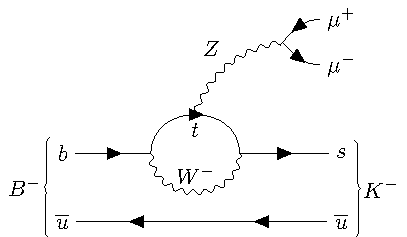
\includegraphics[raise=-20pt]{bminus.pdf} + 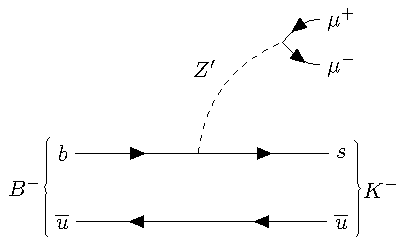
\includegraphics[raise=-20pt]{bminusprime.pdf}
\end{equation}  
Eq (7) shows the suggested sum, with the second diagram showing the new \textit{Z'} that may account for the difference. \\
For this \textit{Z'} to be the solution to the inconsistencies, it must also hold for all other couplings it could affect in the Standard Model.

\section*{Meeting 17/10}
\textit{Taken by Aleksey this week, just a few maths notes.}
\begin{align}
    F_{\mu\nu} &= D_\mu A_\nu - D_\nu A_\mu \\
               &= (\p_\mu - igA_\mu)A_\nu - (\p_\nu - igA_\nu)A_\mu \\
               &= \p_\mu A_\nu - \p_\nu A_\mu - ig[A_\mu,A_\nu] \\
    A_\mu &= \sum_{a=1}^{n^2-1} A_\mu^at^a,~ SU(n) \\
    U(1) &\implies [A_\mu,A_\nu] = 0 
\end{align}
Of course, for the other symmetry groups used in SM, this commutator will not be zero, as Eq (11) implies, which leads to the more complicated Lagrangian for these theories. 
The basic formulation for proving gauge invariance of each group is the same, and follows below, but for the SU(2) and SU(3) groups, Eq (11) must be remembered and applied in addition to the usual methods. 
\begin{align}
    \psi(x) \to \psi'(x) &= e^{ig\alpha(x)} \\
    A_\mu \to A_\mu' &= A_\mu + \p_\mu\alpha(x) \\
    \La &= -\frac14 F_{\mu\nu}F^{\mu\nu} + \bar{\psi}(i\p_\mu\gamma^\mu - m)\psi \\
    \p_\mu \to D_\mu &= \p_\mu - igA_\mu 
\end{align}
All of this is then mashed together into the SM Lagrangian,
\begin{align}
    \La^{SM} &= -\frac14 F_{\mu\nu}F^{\mu\nu}~ \to \text{gauge term} \\ 
             &+ i\bar{\psi}\cancel{D}\psi ~ \to \text{Fermion term} \\
             &+ (D_\mu\phi)^\dagger(D^\mu)\phi - V(\phi) ~ \to \text{Higgs term} \\
             &- Y_{ij}\bar{\psi}_i\phi\psi_j + h.c. ~ \to \text{Yukawa term} \\
             & SU_c(3)\otimes SU(2)_L\otimes U(1)
\end{align}
Very reduced form, most terms can be largely expanded, i.e.
\begin{align}
    -\frac14 F_{\mu\nu}F^{\mu\nu} &= \underbrace{-\frac14 G_{\mu\nu}G^{\mu\nu}}_{SU_c(3)} - \underbrace{\frac14 F_{\mu\nu}F^{\mu\nu}}_{SU(2)_L} - \underbrace{\frac14 B_{\mu\nu}B^{\mu\nu}}_{U(1)} \\
    G_{\mu\nu} &= D_\mu A_\nu - D_\nu A_\mu \\
    D_\mu &= \p_\mu - igA_\mu,\; A_\mu = \frac12 A_\mu^a\lambda^a,\; a = 1,\dots,8 \\
    [A_\mu^a\lambda^a,A_\nu^a\lambda^a] &\neq 0
\end{align}
\end{document}












